\documentclass[%
12pt,
master,  % тип документа
natbib,      % использовать пакет natbib для "сжатия" цитирований
subf,        % использовать пакет subcaption для вложенной нумерации рисунков
substylefile = spbu.rtx,
href,        % использовать пакет hyperref для создания гиперссылок
colorlinks,  % цветные гиперссылки
%fixint,     % включить прямые знаки интегралов
]{disser}

\usepackage[
  a4paper, mag=1000,
  left=2.5cm, right=1cm, top=2cm, bottom=2cm, headsep=0.7cm, footskip=1cm
]{geometry}


\usepackage[colorinlistoftodos]{todonotes}

\usepackage[intlimits]{amsmath}
\usepackage{amssymb,amsfonts}

\usepackage[T2A]{fontenc}
\usepackage[utf8]{inputenc}
%\usepackage[cp1251]{inputenc}
\usepackage[english,russian]{babel}
%\usepackage[backend = biber]{biblatex}
\ifpdf\usepackage{epstopdf}\fi
\usepackage[autostyle]{csquotes}
\bibliographystyle{utf8gost705u}
%\bibliographystyle{gost2008}
%\usepackage[backend=biber, babel=other, style=gost-authoryear]{biblatex}
%\bibliographystyle{gost780s}

% Шрифт Times в тексте как основной
%\usepackage{tempora}
% альтернативный пакет из дистрибутива TeX Live
%\usepackage{cyrtimes}

% Шрифт Times в формулах как основной
%\usepackage[varg,cmbraces,cmintegrals]{newtxmath}
% альтернативный пакет
%\usepackage[subscriptcorrection,nofontinfo]{mtpro2}

% Плавающие рисунки "в оборку".
\usepackage{wrapfig}

% Номера страниц снизу и по центру
%\pagestyle{footcenter}
%\chapterpagestyle{footcenter}

% Точка с запятой в качестве разделителя между номерами цитирований
%\setcitestyle{semicolon}

% Использовать полужирное начертание для векторов
\let\vec=\mathbf

% Включать подсекции в оглавление
\setcounter{tocdepth}{2}

\graphicspath{{fig/}}

\begin{document}
% Переопределение стандартных заголовков
%\def\contentsname{Содержание}
%\def\conclusionname{Выводы}
%\def\bibname{Литература}

%
% Титульный лист на русском языке
%

\institution{%
	Санкт-Петербургский государственный университет \\
	Прикладная математика и информатика \\
	Статистическое моделирование
}

% Имя лица, допускающего к защите (зав. кафедрой)
% \apname{ФИО зав. кафедрой}

\title{Отчет о научно-исследовательской работе}

\topic{\normalfont\scshape%
	Обнаружение разладки во временных рядах показов мобильной
рекламы}

% Автор
\author{Мерзляков Климент Викторович}
% Группа
\group{Студента группы 17.М03-мм}

% Научный руководитель
\sa {Н.\,Э.~Голяндина}
\sastatus{к.\,ф.-м.\,н., доцент}


% Рецензент
% \rev      {П.\,П.~Петров}
% \revstatus{к.\,ф.-м.\,н., доцент}

% Город и год
\city{Санкт-Петербург}
\date{\number\year}

\maketitle

%%
%% Titlepage in English
%%
%
%\setlength\thirdskip{0pt}
%
%\institution{Name of Organization}
%
%% Approved by
%\apname{Professor S.\,S.~Sidorov}
%
%\title{Diploma Thesis}
%
%% Topic
%\topic{Dummy Title}
%
%% Author
%\author{Author's Name} % Full Name
%\group{} % Study Group
%
%% Scientific Advisor
%\sa       {I.\,I.~Ivanov}
%\sastatus {Professor}
%
%% Reviewer
%\rev      {P.\,P.~Petrov}
%\revstatus{Associate Professor}
%
%% Consultant
%\con{}
%\conspec{}
%\constatus{}
%
%% City & Year
%\city{Saint Petersburg}
%\date{\number\year}
%
%\maketitle[en]

% Содержание
\tableofcontents

% Введение
% \input{intro}

\nocite{*}



\intro

Рекламной сетью называют некоторую площадку или систему, которая является посредником между рекламодателями и собственниками рекламных мест --- владельцев сайтов, мобильных приложений и каких-либо других пространств, где можно размещать рекламу.

В интернет-рекламе взаимодействие рекламной сети с пользователем можно описать следующей последовательностью событий. При выполнении некоторых условий (например, пользователь открыл мобильное приложение) с устройства пользователя отправляется запрос на показ рекламы. Если запрос удовлетворяется, то происходит событие „показ“, то есть пользователь непосредственно видит рекламу. После этого может произойти событие „клик“ и далее какое-либо целевое действие. В мобильной интернет-рекламе „показ“ является одним из ключевых событий, поскольку он отражает количество рекламы доставленное до конечного пользователя.

Рекламные интернет-сети являются интересным объектом для исследования с точки зрения обнаружения разладки, поскольку все показатели отслеживаются с точностью до секунды, происходит большое количество событий, а так как рекламные сети, как правило, работают на международном рынке, то существует возможность тестировать гипотезы на большом количестве различных временных рядов.

Одной из текущих проблем, стоящих перед рекламными сетями --- это низкая скорость реагирования на любые резкие изменения текущего состояния. Такие изменения отражаются в данных в виде аномальных значений, резких всплесков и внезапных изменений тренда. Проблема заключается в том, что показателей требующих отслеживания могут быть десятки, при этом на каждый показатель может влиять большое количество факторов. Поэтому зачастую, чтобы локализовать и устранить проблему, требуется просмотреть сотни графиков. Отсюда следует, что наличие качественного метода обнаружения разладки каждого показателя по каждому измерению позволило бы не только существенно сэкономить ресурсы, но и в целом повысить эффективность бизнеса. Поэтому главной задачей данной работы является разработка методики обнаружения разладки. В работе будут использоваться фактические данные одной из работающих рекламных сетей для построения модели данных.

Цель работы --- сравнить методы обнаружения разладки на модельных данных, по виду и структуре похожих на реальные, и выработать рекомендации по использованию методов обнаружения разладки для реальных данных. В связи с этим, структура работы следующая: в первой главе описываются способы оценки параметров модели ряда, предлагается модель сигнала ряда, а также способ моделирования разладок разных видов. Помимо этого в первой главе описываются методы обнаружения разладки и предлагается способ оценки качества этих методов. Во второй, практической, главе происходит подбор параметров модели сигнала в реальных данных, генерируются искусственные ряды, применяются методы описанные в первой главе к этим рядам, сравнивается качество этих методов с рекомендациями в выводах.


% Глава 2
\chapter{Обнаружение разладки во временных рядах}

\section{Построение модели данных}\label{section:data_modeling}

Реальные данные интернет-рекламы имеют стабильную дневную периодичность (на рисунке ~\ref{fig:examples_day} приведен пример типичной почасовой динамики в рамках дня). По более длинному ряду, изображенному на рисунке ~\ref{fig:examples_month}, видно, что в данных время от времени возникают разладки разных видов, при этом сам ряд имеет мультипликативный характер (с изменением среднего уровня ряда пропорционально меняется и амплитуда колебаний). В реальных временных рядах достаточно сложно разметить наличие разладок --- зачастую сложно отделить разладку от шума. Поэтому вместо разметки реальных рядов мы будем моделировать искусственные ряды, похожие на ряды данных интернет-рекламы с определенным шумом и разладками в известных местах.

\begin{figure}[!hhh]
	\begin{center}
		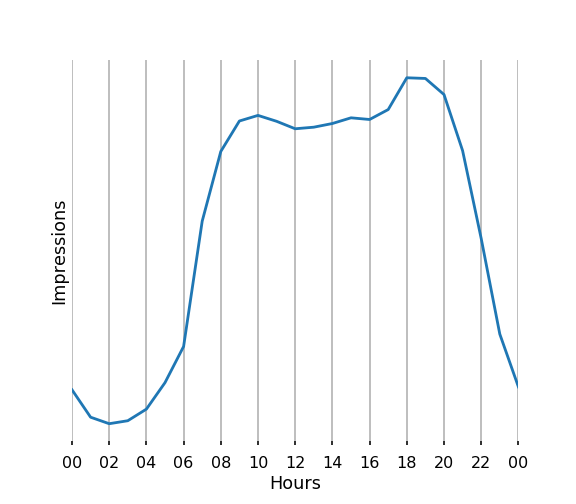
\includegraphics[width=12cm]{examples_day}
	\end{center}
	\vspace{-5mm}\caption{Пример количества показов рекламы за сутки}
	\label{fig:examples_day}
\end{figure}
 
\begin{figure}[!hhh]
	\begin{center}
		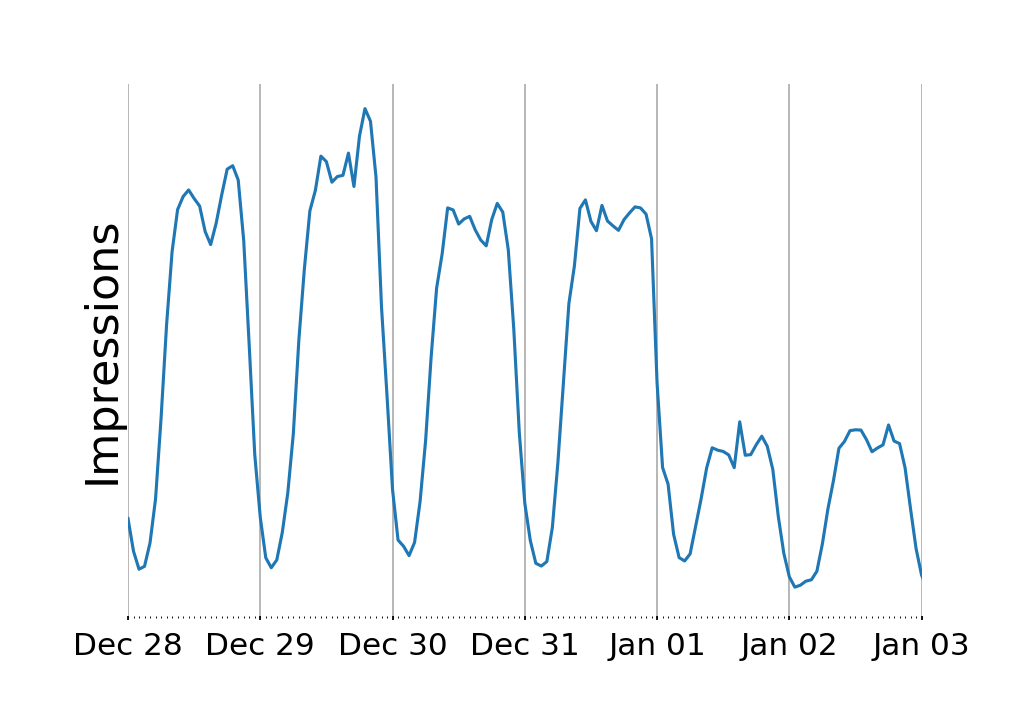
\includegraphics[width=12cm]{cp_mean_2}
	\end{center}
	\vspace{-5mm}\caption{Пример количества показов рекламы с разладкой за неделю}
	\label{fig:examples_month}
\end{figure}

Обозначим временной ряд $Y = (y_1, \dots, y_n)$. Наблюдаемые значения ряда можно представить в виде суммы компонент:
\begin{equation*}
Y = T + S + E ,
\end{equation*}
где  $ T = (t_1, \dots, t_n) $ компонента-тренд, $ S = (s_1, \dots, s_n) $ периодическая компонента, $ E = (\epsilon_1, \dots, \epsilon_n) $ остатки или шум.
Для каждой из этих компонент требуется построить модель. Модель можно задать следующим образом:
\begin{equation*}
t_i = c, \quad i = 1, \dots, n, 
\end{equation*}
\begin{equation*}
s_i = \sum_{j=1}^{J}{A_j \cos \left( \frac{2\pi}{a_j} i + \phi_j \right)}, \quad i = 1, \dots, n,
\end{equation*}
\begin{equation*}
\epsilon_i \sim N(0, \sigma^2), \quad i = 1, \dots, n, 
\end{equation*}
где $i$ --- индекс элемента ряда; $j$ --- индекс косинуса в периодической компоненте; J --- количество косинусов в периодической компоненте; $c$ --- константа; $A_j$ --- амплитуда $j$-го косинуса; $a_j$ --- период $j$-го косинуса; $\phi_j$ --- фаза $j$-го косинуса.

%Ряды, модель которых мы хотим построить, имеют мультипликативность (амплитуда колебаний меняется пропорционально изменению тренда). Такого эффекта можно достичь, взяв экспоненту от исходной модели ряда:
%\begin{equation*}
%Y^{\mathrm{(mult)}} = e^{Y}. 
%\end{equation*}

В данной работе мы будем проверять качество методов для двух наиболее часто встречающихся типов разладки --- разладка в среднем и локальная разладка (в одной точке).

%Построим модель разладки, исходя из следующего:
%\begin{itemize}
%	\item Разладка только в одной точке ряда;
%	\item Разладка заключается в сдвиге;
%\end{itemize}
Формально модель разладки можно описать так: пусть $\tau$ --- точка (индекс) разладки, тогда тренд с разладкой обозначим $ \tilde{T} = (\tilde{t_1}, \dots, \tilde{t_n}) $. В случае разладки в среднем $\tilde{t_i} будет принимать следующий вид:$
\begin{equation*}
\tilde{t_i} =
	\begin{cases}
		t_i, & i < \tau, \\
		t_i + \delta^{(mean)}, & i \geqslant \tau,
	\end{cases}
\end{equation*}
где $ \delta^{(mean)} $  --- значение разладки. Чтобы разладка была заметна, введем ещё минимальное допустимое значение разладки $\delta_{min}^{(mean)}$.
\begin{equation*}
\delta^{(mean)} = \max(\delta^{(mean)*}, \delta_{min}^{(mean)} ),
\end{equation*}
\begin{equation*}
\delta^{(mean)*} \sim N(\mu^{\mathrm{(cp\_mean)}}, \sigma^{2\mathrm{(cp\_mean)}}).
\end{equation*}
В случае локальной разладки модель разладки будет выглядеть следующим образом:
\begin{equation*}
\tilde{t_i} =
	\begin{cases}
		t_i, & i \neq \tau, \\
		t_i + \delta^{(local)}, & i = \tau,
	\end{cases}
\end{equation*}
со схожим ограничением на минимальное значение разладки:
\begin{equation*}
\delta^{(local)} = \max(\delta^{(local)*}, \delta_{min}^{(local)} ),
\end{equation*}
\begin{equation*}
\delta^{(local)*} \sim N(\mu^{\mathrm{(cp\_local)}}, \sigma^{2\mathrm{(cp\_local)}}).
\end{equation*}
%Значение разладки является случайной величиной с некоторым распределением. В данной работе значение разладки будет иметь нормальное распределение $ \delta^* \sim N(\mu^{\mathrm{(cp)}}, \sigma^{2\mathrm{(cp)}})  $, с некоторой вероятностью возникновения $ \rho $:
%
%\begin{equation*}
%\delta = \begin{cases}
%    		\delta^*, & \textrm{с вероятностью } \rho, \\
%  		0, & \textrm{с вероятностью } 1 - \rho.
%	\end{cases} 
%\end{equation*}
%Таким образом, $\delta$ является случайной величиной с распределением-смесью. При этом точка разладки  $\tau$ тоже может являться случайной величиной с равномерным распределением на $ [n_0, \dots, n - n_0 ] $, где $ n_0 $ --- самая первая возможная точка разладки, которая задается параметром. $n_0$ введена намеренно, чтобы разладка при моделировании не возникала в первых и последних точках ряда. Однако в данной работе, для упрощения оценки качества методов $\tau$  будет не случайной величиной, а фиксированным параметром, то есть $\tau = n_0$.
Таким образом, моделируемый ряд с разладкой будет иметь следующий вид:
%\begin{equation*} Y = e^{\tilde{T} + S + E}.  \end{equation*}
\begin{equation*}
\tilde{Y} = \tilde{T} + S + E. 
\end{equation*}
В результате модель временного ряда имеет следующие параметры: $ \{A\}_{j=1}^J$, $ \{a\}_{j=1}^J$, $ \{\phi\}_{j=1}^J$, $\sigma, c $, а модель разладки имеет еще три параметра: $ \mu^{\mathrm{(cp)}}, \sigma^{\mathrm{(cp)}}, \delta_{min} $.


\section{Оценка параметров модели}\label{section:parameters_estimation}

В  \cite{Golyandina2018}  описан подход к определению параметров модели временного ряда $ \{A\}_{j=1}^J$,  $\{a\}_{j=1}^J$,  $\{\phi\}_{j=1}^J$, основанный на траекторной матрице ряда. Предполагая, что периодическая компонента ряда управляется линейной рекуррентной формулой, можно записать её в виде $s_i = \sum_{j=1}^r c_j \mu_j^n = \sum_ta_t\rho_t^n \cos(2\pi \omega_t n + \phi_t)$, $\mu_j = \rho_j e^{2\pi i \omega_j}$, где $u_j$ --- корни характеристического полинома. 

%В целом, сигнальные корни характеристического полинома, управляемого линейной рекуррентной формулой позволяют оценить сигнальные параметры $\mu_j$. Однако, мы должны уметь отделять сигнальные корни от избыточных. Обычно сигнальные корни минимальной реккурентной формулы имеют максимальные значения по модулю. Поэтому можно найти корни, упорядочить их по убыванию и взять первые $r$ штук. Однако такой способ не гарантирует, что сигнальные корни будут упорядочены. Поэтому существует другой 

Оценить сигнальные параметры $\mu_j$ позволяет метод, который называется ESPRIT \cite{esprit}.


Обозначим $\{U_1, \dots, U_r \}$ ортонормированный базис оцениваемого подпространства, интересующей компоненты. Такой базис можно оценить, например, с помощью метода SSA, где $r$ будет параметром, обозначающий каким количеством компонент мы оцениваем сигнал временного ряда.
%Составим матрицы $\textbf{P}_x = [\underline{U_1}: \dots : \underline{U_r}]$, $\textbf{Q}_x = [\overline{U_1}: \dots : \overline{U_r}]$, $\textbf{P}_y = [U_1|: \dots : U_r|]$, $\textbf{Q}_y = [|U_1: \dots : |U_r]$, где $(\underline{\cdot})$, $(\overline{\cdot})$, $(\cdot|)$, $(|\cdot)$ обозначают вектор без первой строки, последней строки, первого столбца


 Обозначим $\textbf{P}_r = [U_1 : \dots : U_r ]$, а $\underline{\textbf{P}_r}$ матрица без последней строки, а $\overline{\textbf{P}_r}$  матрица без первой строки. Тогда $\mu_i$ может быть оценено с помощью собственных значений матрицы $\underline{\textbf{P}_r}^{\dagger}\overline{\textbf{P}_r}$, где $\dagger$ обозначает псевдо-инверсию. Соответственно, оцениваемые частоты и являются аргументами $\mu_i$.
%Опишем метод оценки частотных параметров модели, который используется для обнаружения собственных троек на шаге группировки в методе SSA. Два вектора $U^{(1)}$ и $U^{(2)}$ образующие ортогональный базис траекторного пространства экспоненциально модулированного синуса имеют схожие фазы, отличающиеся примерно на $\frac{\pi}{2}$. Пусть $A$ и $B$ определяется как $a_n = \rho^n \sin(2\pi \omega n + \phi)$ и $b_n = \rho^n \cos(2\pi \omega n + \phi)$. Обозначим угол между векторами как $\angle$. Тогда $\omega = \angle  \begin{pmatrix} \begin{pmatrix}a_1\\b_1\end{pmatrix}, \begin{pmatrix}a_2\\b_2\end{pmatrix} \end{pmatrix} \bigg/ (2\pi).$ Поэтому мы можем оценить частоту используя базисные векотры $U^{(1)}$ и $U^{(2)}$. Поскольку эти векторы имеют немного другую форму, чем $A$ и $B$, можно использовать последовательность углов $\angle  \begin{pmatrix} \begin{pmatrix}u_i^{(1)}\\u_i^{(2)}\end{pmatrix}, \begin{pmatrix}u_{i+1}^{(1)}\\u_{i+1}^{(2)}\end{pmatrix} \end{pmatrix} \bigg/ (2\pi), i = 1, \dots , L - 1,$ и среднее и медиана будет оценкой частоты.

Для упрощения модели, в работе мы исправляем корни $\mu_j$, заменяя их на корни с модулем 1 и точными периодами. Получив оценки частот, можно взять сумму косинусов и синусов с этими частотами как модель и с помощью МНК подобрать параметры амплитуд. Далее, каждую пару синусов и косинусов с одинаковыми частотами можно сгруппировать в один косинус следующим образом:
\begin{equation*}
a_1 \cos(\omega t) + a_2 \sin(\omega t) = a_1 \cos(\omega t) + a_2 \cos(\omega t - \frac{\pi}{2}) = \sqrt{a_1^2 + a_2^2} \cos(\omega t - \arctg(\frac{a_1}{a_2}) ).
\end{equation*}


\section{Методы обнаружения разладки}


Опишем один из подходов к обнаружению разладки. Данный подход не является единственным, хотя заключает в себе широкое разнообразие методов \cite{cp_disser,ruptures}. Как правило, у временного ряда есть некоторая структура (сигнал), которая может быть описана той или иной моделью. Идея подхода заключается в том, что около точки разладки модель плохо описывает временной ряд. Используя некоторую меру ошибки мы можем измерять то, насколько хорошо или плохо описывает выбранная модель реальные данные. Как только ошибка (отклонение модели от реальных данных) превышает заданный порог, метод сигнализирует о разладке.

Можно выделить два типа методов в данном подходе:
\begin{itemize}
	\item Методы на основе прогнозирования
	\item Методы на основе аппроксимации
\end{itemize}

Следует обратить внимание, что исходная модель ряда одна:
\begin{equation*}
Y = T + S + E = c + \sum_{j=1}^{J}{A_j \cos \left( \frac{2\pi}{a_j} i + \phi_j \right)} + \epsilon_i, \quad i = 1, \dots, n.
\end{equation*}
При этом оба типа методов в своей основе будут иметь ту или иную модель ряда $f(x|\theta)$ сигнала для обнаружения разладки, где $\theta$ --- параметры модели. Этих моделей ряда может быть много.
Модель может быть константной ($\theta = (b)$):
\begin{equation*}
f(x | b) = b,
\end{equation*}
либо другой подходящей под наш ряд функцией, один косинус:
\begin{equation*}
f(x | P, p, \chi, b) = P\cos(\frac{2\pi}{p}x + \chi) + b,
\end{equation*}
либо более сложной функцией --- суммой косинусов:
\begin{equation*}
f(x | \{P_j, p_j, \chi_j\}, b) = \sum_{j=1}^JP_j\cos(\frac{2\pi}{p_j}x + \chi_j) + b,
\end{equation*}
и для отдельной проверки модель с трендом:
\begin{equation*}
f(x | c, b) = cx + b.
\end{equation*}

\subsection{Методы на основе аппроксимации}

Пусть $l$ --- чётное вещественное число, называемое шириной окна. При этом  $ 1 < l < n $. С помощью ширины окна из исходного ряда образуется последовательность отрезков $W = \{ w_j \}_{j=1}^k$, где $k = n - l + 1$ --- количество таких отрезков; а $ w_j = (y_j, \dots, y_{j+l-1}) $ --- $j$-ый отрезок. Каждый отрезок  $w_j$  в свою очередь делится на два отрезка одинаковой длины (это возможно, поскольку $l$ четное по условию): $ W^{\mathrm{(left)}} = \{w_j^{\mathrm{(left)}} \}  =  \{(y_j, \dots, y_{j+\frac{l}{2}-1}) \}$ и $W^{\mathrm{(right)}} = \{w_j^{\mathrm{(right)}} \} = \{(y_{j+\frac{l}{2}}, \dots, y_{j+l-1}) \}$.

Таким образом, для каждого ряда $W$ можно сформировать тройки рядов: 
\begin{equation*}
W^{\mathrm{(all)}} = \{w_j^{\mathrm{(all)}} \}_{j=1}^k =  \{(w_j; w_j^{\mathrm{(left)}}; w_j^{\mathrm{(right)}}) \}_{j=1}^k. 
\end{equation*}
Пусть есть функция ошибки $e(\cdot)$, такая что:
\begin{equation*}
e(X) = \min_{\theta}{\sum_{p=1}^m(x_p - f(x_p | \theta))^2 },
\end{equation*}
где $X = (x_1, \dots, x_m)$ ---  вещественный временной ряд длины $m$, а $f(x | \theta)$ --- модель сигнала этого временного ряда с параметрами $\theta$.

%\todo[inline]{Надо ли здесь вводить новое обозначение для временного ряда, если есть уже ряд Y.}

Мера ошибки позволяет нам рассчитать, насколько хорошо аппроксимируется отрезок ряда с помощью выбранной модели. Однако, для обнаружения самой разладки необходимо еще ввести функцию разладки:
\begin{equation*}
f_j = F(w_j^{\mathrm{(all)}} ) = \frac{e(w_j) - e(w_j^{\mathrm{(left)}}) - e(w_j^{\mathrm{(right)}})}{h}, 
\end{equation*}
где $h$ --- значение нормировки, $j = 1, \dots, k$.

Отметим, что значения функции разладки синхронизируются с исходным рядом по последнему индексу окна. То есть $f_1$ соответствует $y_l$, а $f_k $ соответсвует $y_n$. Введем синхронизированную функцию разладки :
\begin{equation*}
q_i =
	\begin{cases}
		f_{i-l+1}, & i \geq l, \\
		0, & i < l.
	\end{cases}
\end{equation*}
Нормирующая константа $h$ нам необходима для того, чтобы приводить значения функции разладки к значениям близким к диапазону от $0$ до $1$, поскольку без нормировки значения функции разладки могут принимать сколь угодно большие значения. Из-за этого без нормировки получается проблематично выбирать адекватные значения порога для метода (непонятно какое значение большое, а какое маленькое). Подход к расчету нормирующей константы является открытой проблемой, поскольку имеются разные варианты её расчета со своими плюсами и минусами.
Например, можно рассчитывать её как ненормированное значение функции разладки на первом отрезке ряда (предполагая, что на этом отрезке не происходило разладок):
\begin{equation*} 
h = e(w_1) - e(w_1^{\mathrm{(left)}}) - e(w_1^{\mathrm{(right)}}) + 1. 
\end{equation*}

Либо, можно проходить скользящим окном начало ряда и рассчитывать ненормированное значение функции разладки для каждого окна и затем усреднять полученные значения. Такой подход помогает избежать ситуаций с выбранным малым окном, когда мы не охватываем всю периодичность одним окном.
\begin{equation*} 
h = \frac{\sum_{j=1}^{v}e(w_j) - e(w_j^{\mathrm{(left)}}) - e(w_j^{\mathrm{(right)}})}{v} + 1, 
\end{equation*}
где $v$ --- сколько отрезков в начале ряда мы используем для расчета $h$.


Для наглядности, на рисунке ~\ref{fig:approximation_example_1} приведен пример расчета ошибки на одном левом ряде $ w_j^{\mathrm{(left)}} $ и на одном правом ряде $ w_j^{\mathrm{(right)}} $. А на рисунке ~\ref{fig:approximation_example_2} показан пример расчет ошибки на одном общем ряде (в который входит и левая и правая части). А на рисунке ~\ref{fig:approximation_example_3} изображен пример расчета функции разладки с помощью скользящего окна.


\begin{figure}[!hhh]
	\begin{center}
		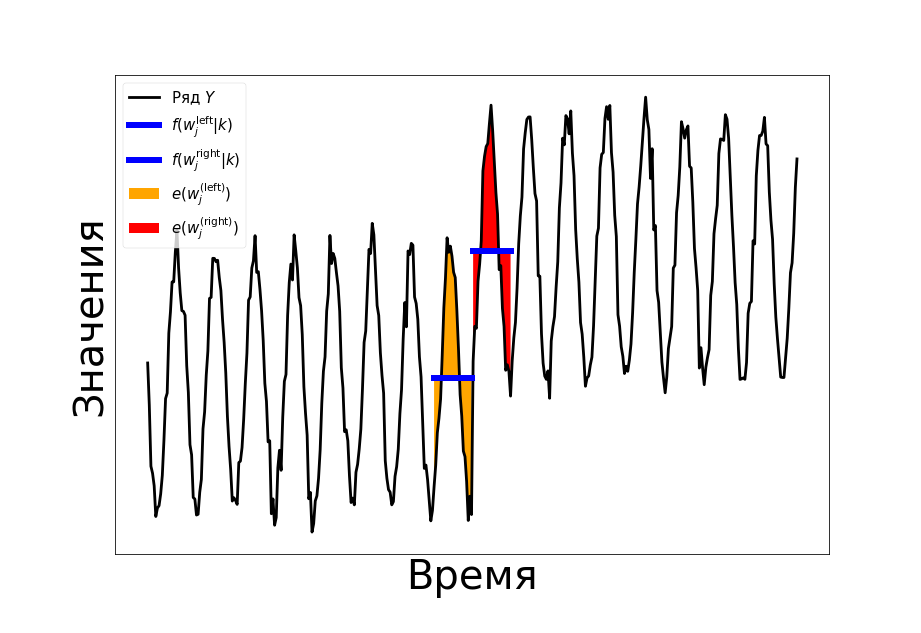
\includegraphics[width=12cm]{approaches_second_2_ru}
	\end{center}
	\vspace{-5mm}\caption{Пример промежуточного расчета ошибки методом аппроксимации}
	\label{fig:approximation_example_1}
\end{figure}

\begin{figure}[!hhh]
	\begin{center}
		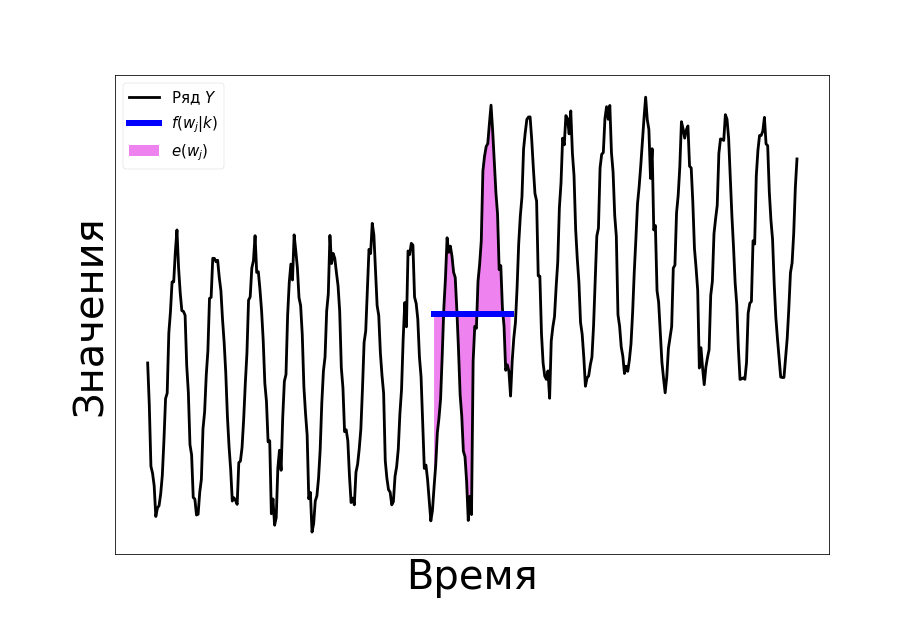
\includegraphics[width=12cm]{approaches_second_3_ru}
	\end{center}
	\vspace{-5mm}\caption{Пример промежуточного расчета ошибки методом аппроксимации, продолжение.}
	\label{fig:approximation_example_2}
\end{figure}

\begin{figure}[!hhh]
	\begin{center}
		\includegraphics[width=12cm]{approaches_second_4_ru}
	\end{center}
	\vspace{-5mm}\caption{Пример расчета функции разладки с помощью скользящего окна}
	\label{fig:approximation_example_3}
\end{figure}


Итого, взяв ряд $Y$, мы «скользим» по нему окном ширины $l$ и рассчитываем значения функции разладки $F()$ для каждого из получаемых отрезков $W^{\mathrm{(all)}}$. Функция разладки начинает расти в окрестности точки разладки $\tau$, следовательно можно задать некий порог $\gamma$, такой что при превышении функции разладки этого порога в какой-то точке $\hat{\tau}$ будем считать, что разладка обнаружена в этой точке.

В результате, в данных методах нужно задавать следующие параметры: ширину окна $l$, модель $f$ и порог $\gamma$.

\subsection{Методы на основе прогнозирования}

Методы на основе прогнозирования очень похожи на методы с использованием аппроксимации. Суть их заключается в том, что мы строим прогноз на несколько точек ряда вперед и считаем отклонение фактических значений от прогнозных. В случае, если отклонение выше заданного порога, метод обнаруживает разладку.
Формально, оставаясь в тех же обозначениях, есть всё та же ширина окна $l$ (однако $l$ в данном случае может быть нечетным) и последовательность отрезков $W = \{ w_j \}_{j=1}^k$. Каждый отрезок  $w_j$ делится в этом методе на два ряда не обязательно одинаковой длины. Введем индекс $g$, который будет указывать в какой точке ряда $w_j$ он будет разделен на два. Таким образом, формируется набор из пар рядов:  $ W^{\mathrm{(left)}} = \{w_j^{\mathrm{(left)}} \}  =  (y_j, \dots, y_{j+g-1})$ и $W^{\mathrm{(right)}} = \{w_j^{\mathrm{(right)}} \} = (y_{j+g}, \dots, y_{j+l})$. Ключевое отличие от методов аппроксимации заключается в том, что вместо расчета мер ошибок на тех же рядах, на которых подбирались параметры моделей (параметры модели и ошибка для левого отрезка оценивались на левом отрезке и так для всех трех моделей $w_j^{(all)}$), мы оцениваем параметры $\theta$ модели $f(x|\theta)$ на ряде $ w_j^{\mathrm{(left)}} $, делаем прогноз на $ l - g $ точек и рассчитываем функцию ошибки $ e(\cdot) $ на ряде $ w_j^{\mathrm{(right)}} $. При этом функция разладки принимает следующий вид:
	\begin{equation*}
	 f_j = F(w_j^{\mathrm{(right)}}) = \frac{e(w_j^{\mathrm{(right)}})}{h}.
	 \end{equation*}
В остальном данные методы ничем не отличаются от методов на основе аппроксимации. Следовательно, синхронизированная функция разладки $q_i$ синхронизируется с исходным рядом аналогичным образом.

Для наглядности, на рисунке ~\ref{fig:predicition_example_1} приведен пример расчета ошибки с помощью метода прогнозирования на одном ряде  $ w_j^{\mathrm{(right)}} $. А на рисунке ~\ref{fig:predicition_example_2} показан пример расчета функции разладки $ F(w_j^{\mathrm{(right)}}) $ для всего ряда.

\begin{figure}[!hhh]
	\begin{center}
		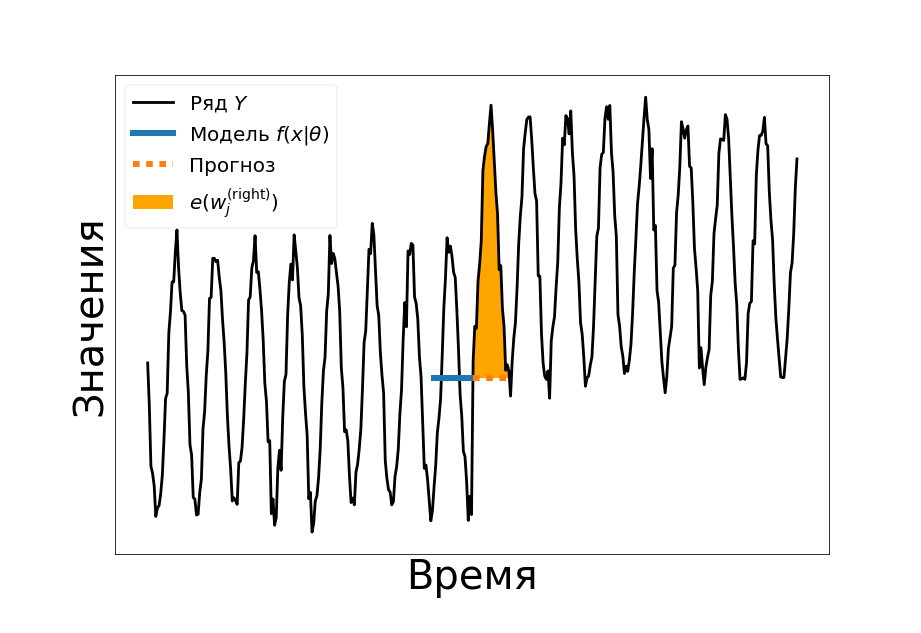
\includegraphics[width=12cm]{approaches_first_4_ru}
	\end{center}
	\vspace{-5mm}\caption{Пример расчета ошибки методом прогнозирования}
	\label{fig:predicition_example_1}
\end{figure}

\begin{figure}[!hhh]
	\begin{center}
		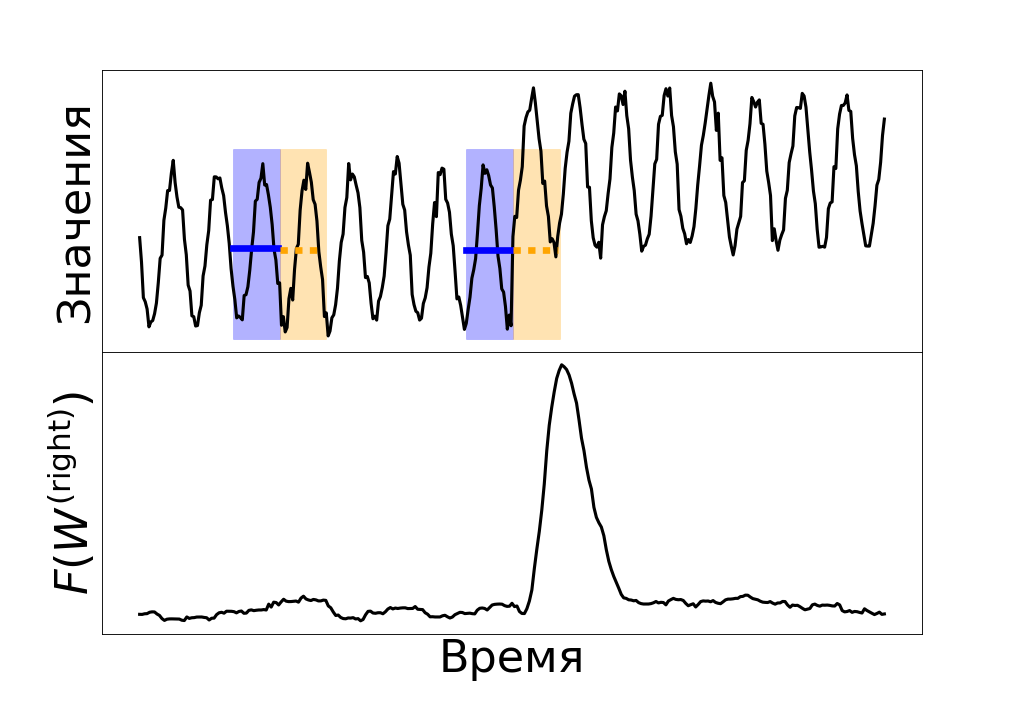
\includegraphics[width=12cm]{approaches_first_6_ru}
	\end{center}
	\vspace{-5mm}\caption{Пример расчета функции разладки с помощью скользящего окна}
	\label{fig:predicition_example_2}
\end{figure}

В методах прогнозирования нужно задавать следующие параметры: ширину окна $l$, модель $f$, индекс разделения окна (по сути с помощью него определяется на основе какого количества точек подбираются параметры модели, а на сколько точек происходит прогноз) $g$ и порог $\gamma$.

%\todo[inline]{Есть смысл в дальнейшем переписать аппроксимацию (l не обязательно четное, а функции ошибок делятся на ширину. Тогда получится универсальная запись для прогнозирования и для аппроксимации)}

\section{Оценка качества}

В рамках данной работы мы разрабатываем систему своевременного оповещения о разладках во временных рядах. При такой постановке задачи важны две характеристики: точность обнаружения разладки и скорость обнаружения разладки. Поскольку мы используем моделированные данные, то мы точно знаем в каких из смоделированных нами рядов произошла разладка, а в каких разладки не было. Более того, мы точно знаем момент разладки. Благодаря этому, мы можем строить матрицы ошибок классификации и считать метрики качества. При этом важно обнаружить разладку не позднее какого-то срока, иначе оповещение о разладке будет несвоевременным. Поэтому мы фиксируем точку разладки $\tau$ и вводим параметр допустимой задержки $d$.
%Также, чтобы получать разумные результаты оценки методов, мы будем исходить из того, что метод может обнаруживать сколь угодно много разладок, в то время как фактическая разладка будет происходить только в одном месте (либо не происходить вовсе). Такая поправка введена намерено, в частности во избежания случаев, когда метод с низким значением порога $\gamma$ будет останавливаться практически сразу, из-за чего матрицы сопряженности становится проблематично интерпретировать.

% Таким образом, после каждого применения метода обнаружения разладки мы получаем вектор точек разладок $ \mathrm{\hat{T}} = (\hat{\tau}_1, \cdots, \hat{\tau}_q) $, где $q$ --- количество разладок, обнаруженное методом. Стоит отметить, что $q$ может быть равно нулю.

Следовательно, в рамках данной работы мы будем строить классифицирующее правило:
\begin{equation*}
a(Y) = 
	\begin{cases}
		1, & f_j \geq \gamma \text{ и } \tau-l \leq j \leq \tau-l+d-1, \\
		0, & \text{иначе},
	\end{cases}
\end{equation*}
где $0$ означает, что разладки нет (negative), $1$ означает, что разладка есть (positive).
%f_j < \gamma \text{ или }  j < \tau-l \text{ или }  j > \tau-l+d
Таким образом, метод будет определять, либо не определять разладку в заданном диапазоне в зависимости от задаваемого порога $\gamma$.

Исходя из этого возможны четыре варианта:

%\begin{itemize}
%	\item Разладка произошла и метод обнаружил точку разладки \textbf{после} фактической точки $\tau$, но не слишком поздно, то есть не позднее, чем $\tau + u$, где $u$ параметр. Параметром $u$ мы задаем приемлемую для нас задержку в обнаружении разладки. Такая ситуация попадает под категорию True positive.
%	\item Разладка произошла и метод не обнаружил точку разладки в диапазоне $(\tau, \cdots, \tau + u)$. Это случай False negative.
%	\item Метод обнаружил разладку там, где ее не было. То есть либо за пределами $(\tau, \cdots, \tau + u)$, либо когда разладки вообще не было в ряде. Это ситуация False positive.
%	\item Разладки не было и метод не обнаружил разладку. Это случай True negative.
%\end{itemize}

%\begin{itemize}
%	\item Разладка произошла и метод обнаружил точку разладки \textbf{после} фактической точки $\tau$, но не слишком поздно, то есть не позднее, чем $\tau + u$, где $u$ параметр. Параметром $u$ мы задаем приемлемую для нас задержку в обнаружении разладки. Такая ситуация попадает под категорию True positive.
%	\item Разладка произошла и метод не обнаружил точку разладки в диапазоне $(\tau, \cdots, \tau + u)$. Это случай False negative.
%	\item Метод обнаружил разладку в ряде без разладки. Это ситуация False positive.
%	\item Разладки не было и метод не обнаружил разладку. Это случай True negative.
%\end{itemize}

\begin{itemize}
	\item Разладка произошла и метод обнаружил точку разладки в диапазоне $(\tau, \cdots, \tau+d-1)$. Такая ситуация попадает под категорию True positive.
	\item Разладка произошла и метод не обнаружил точку разладки в диапазоне $(\tau, \cdots, \tau+d-1)$. Это случай False negative.
	\item Метод обнаружил разладку в диапазоне $(\tau, \cdots, \tau+d-1)$ в ряде без разладки. Это ситуация False positive.
	\item Разладки не было и метод не обнаружил разладку в диапазоне $(\tau, \cdots, \tau+d-1)$. Это случай True negative.
\end{itemize}



Договорившись о таком способе оценки качества, можно строить ROC-кривые (изменяя порог $\gamma$) для разных методов обнаружения разладки, сравнивая как работают те или иные методы в контролируемой среде эксперимента.

ROC-кривая --- график, позволяющий оценить качество бинарной классификации. Он отображает соотношение между долей верно-положительно классифицированных наблюдений от общего количества положительных классов, и долей ложно-отрицательно классифицированных наблюдений от общего количества отрицательных наблюдений при варьировании порога $\gamma$.
Другими словами, ROC кривая это график, где по оси ординат откладывается TPR (англ. True Positive Rate), а по оси абсцисс откладывается FPR (англ. False Positive Rate). При этом каждая точка является значением TPR и FPR для какого-то конкретного значения порога.
\begin{equation*}
TPR (\gamma) = \frac{\text{Верно-положительные классификации}}{\text{Все положительные наблюдения}},
\end{equation*}
\begin{equation*} 
FPR(\gamma) = \frac{\text{Ложно-отрицательные классификации}}{\text{Все отрицательные наблюдения}}.
\end{equation*}
Для сравнения качества методов мы будем пользоваться метрикой ROC-AUC, которая является ничем иным как площадью по ROC-кривой. ROC-AUC удобно использовать, поскольку она удобно отражает качество метода одним числом. Но помимо оценки самого ROC-AUC нам бы хотелось оценить доверительный интервал, в который попадает ROC-AUC с заданным уровнем значимости. В статье \cite{roc-confidence} предлагают способ оценки стандартного отклонения ROC-AUC. Оценка эта исходит из того, что для больших выборок значение ROC-AUC имеет нормальное распределение. Поэтому доверительный интервал с уровнем доверия $1 - \alpha$ можно посчитать следующим образом:
\begin{equation*}
AUC \pm z_{\frac{\alpha}{2}} \sigma(AUC),
\end{equation*}
где $z$ --- стандартизованная оценка, а $1 - \alpha$ --- уровень значимости.
Способ оценки стандартного отклонения предложен авторами статьи:
\begin{equation*}
\sigma(AUC) = \sqrt{\frac{AUC(1 - AUC) + (N_p - 1)(Q_1 - AUC^2) + (N_n-1)(Q_2 - AUC^2)}{N_pN_n}}, \end{equation*}
где $N_p$ --- количество положительных наблюдений в выборке (в нашем случае количество рядов с разладкой), $N_n$ --- количество негативных наблюдений в выборке (количество рядов без разладки),
\begin{equation*} 
Q_1 = \frac{AUC}{2 - AUC},
\end{equation*}
\begin{equation*}
Q_2 = \frac{2AUC^2}{1 + AUC}.
\end{equation*}


\chapter{Численные эксперименты}


\section{Моделирование данных}

На рисунке ~\ref{fig:examples_long_ts} представлен пример реальных почасовых данных показов рекламы за пять недель. В рамках суток данные имеют два типа структуры --- структуру буднего дня (рисунок ~\ref{fig:examples_day}) и структуру выходного дня (рисунок ~\ref{fig:examples_weekend}). Следовательно, моделировать будние и выходные дни лучше отдельно, в этой работе мы сфокусируемся на выходных днях, однако аналогичные действия применимы и к будним дням. Попробуем убрать из реальных данных будние дни и „склеить“ выходные дни в один ряд. Получившийся ряд изображен на рисунке ~\ref{fig:examples_long_weekends}.
Мы можем смоделировать данный ряд используя подход, описанный в разделе ~\ref{section:data_modeling}. 
Процедура оценки параметров SSA определила следующие параметры модели ряда. Ряд можно смоделировать четырьмя косинусами $J=4$ с периодами $a_1 = 23.93 \approx 24$, $a_2 = 11.99 \approx 12$, $a_3 = 7.99 \approx 8$, $a_4 = 5.99 \approx 6$ (это логично, поскольку наши данные имеют суточные колебания). Оценка амплитуд данным методом получилась $A_1 = 1.00$, $A_2 = 0.39$, $A_3 = 0.13$, $A_4 = 0.11$. А фазы косинусов получились $\phi_1 = 2.78 \approx \frac{8\pi}{9}$, $\phi_2 = 1.55 \approx \frac{\pi}{2}$, $\phi_3 = -1.56 \approx -\frac{\pi}{2}$, $\phi_4 = -2.95 \approx -\frac{15\pi}{16}$. Таким образом, модель периодической составляющей $s_i$ нашего ряда можно записать в следующем виде:
\begin{equation*}
s_i = 1.00\cos(\frac{2\pi}{24}i + \frac{8\pi}{9}) + 
                    0.39\cos(\frac{2\pi}{12}i + \frac{\pi}{2}) + 
                    0.13\cos(\frac{2\pi}{8}i - \frac{\pi}{3}) + 
                    0.11\cos(\frac{2\pi}{6}i - \frac{15\pi}{16}), \quad i = 1, \dots, n.
\end{equation*}
Длину ряда зафиксируем $n = 400$. Значение тренда выберем нулевым: $c = 0$, то есть $t_i = 0, i = 1,\cdots, n$; параметры шума возьмем $\mu = 0, \sigma = 0.1$.

В результате, моделируемые ряды получились внешне достаточно похожими на реальные данные. На рисунке ~\ref{fig:real_vs_modelled} изображено сравнение реальных данных (из которых предварительно вычли среднее значение и отнормировали) и смоделированных по модели, описанной выше.

\begin{figure}[!hhh]
	\begin{center}
		\includegraphics[width=12cm]{real_vs_modelled}
	\end{center}
	\vspace{-5mm}\caption{Сравнение реальных отнормированных данных и смоделированных}
	\label{fig:real_vs_modelled}
\end{figure}


\begin{figure}[!hhh]
	\begin{center}
		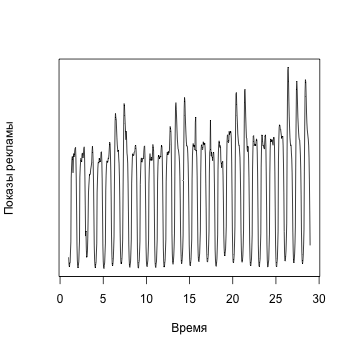
\includegraphics[width=12cm]{examples_long_ts}
	\end{center}
	\vspace{-5mm}\caption{Пример реальных данных показов рекламы}
	\label{fig:examples_long_ts}
\end{figure}

\begin{figure}[!hhh]
	\begin{center}
		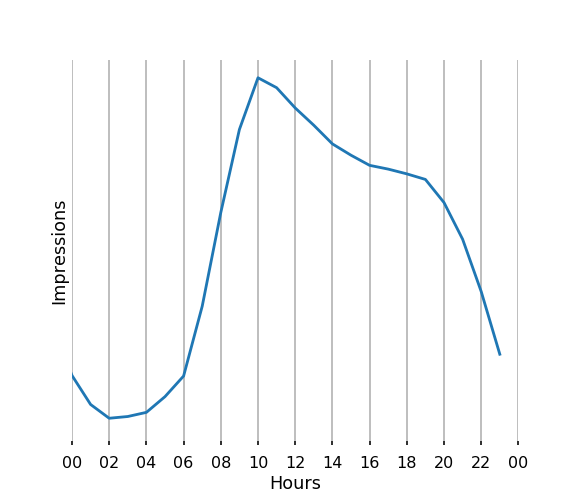
\includegraphics[width=12cm]{examples_weekend}
	\end{center}
	\vspace{-5mm}\caption{Пример количества показов рекламы в выходной день}
	\label{fig:examples_weekend}
\end{figure}

\begin{figure}[!hhh]
	\begin{center}
		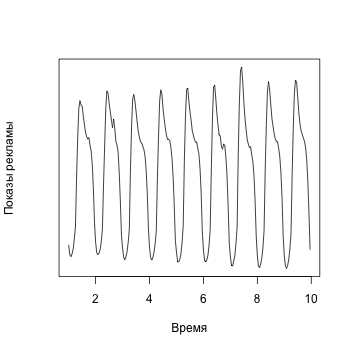
\includegraphics[width=12cm]{examples_long_weekends}
	\end{center}
	\vspace{-5mm}\caption{Реальные данные показов рекламы без будних дней}
	\label{fig:examples_long_weekends}
\end{figure}



Таким образом, модель для генерации ряда имеет следующий вид:
\begin{equation*} y_i = s_i + N(\mu = 0, \sigma^2 = 0.01).\end{equation*}
Моделировать будем 100 рядов (50 с разладкой и 50 без). Величины разладки $\delta^{(mean)*} \sim N(\mu = 0,\sigma^2 = 0.04)$, $\delta^{(local)*} \sim N(\mu = 0,\sigma^2 = 1)$. Минимальные допустимые значения разладок выберем $\delta^{(mean)*}_{min} = 0.3$, $\delta^{(local)*}_{min} = 0.5$. Место возникновения разладки зададим в середине ряда $\tau = 216$, а допустимых задержек выберем несколько $d = (4, 24, 48)$.

Пример сгенерированного ряда с разладкой показан на рисунке ~\ref{fig:data_modeling_example_2}.

\begin{figure}[!hhh]
	\begin{center}
		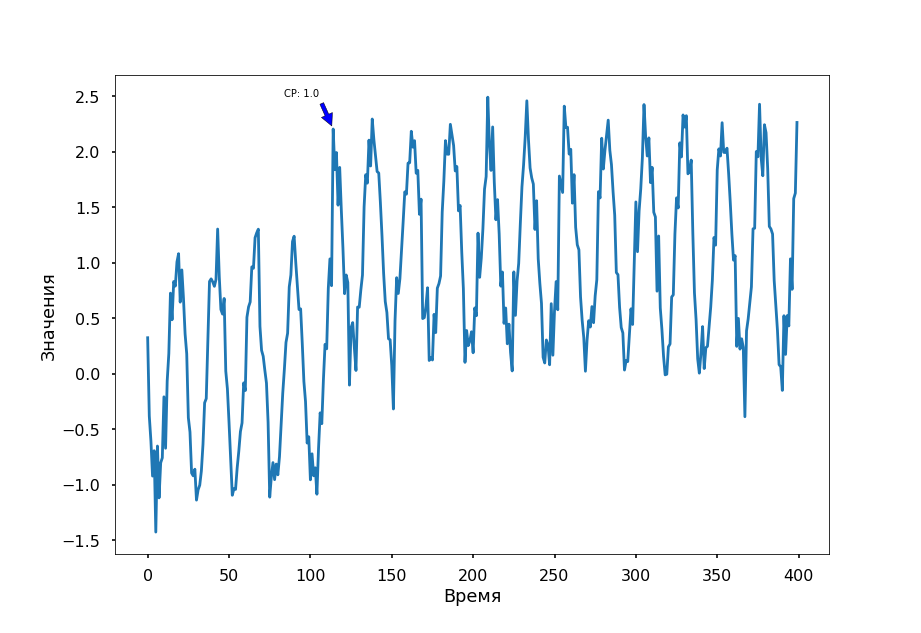
\includegraphics[width=12cm]{data_modeling_example_2}
	\end{center}
	\vspace{-5mm}\caption{Пример сгенерированного ряда с разладкой}
	\label{fig:data_modeling_example_2}
\end{figure}

% Поскольку реальные данные имеют мультипликативный характер, то мы будем брать экспоненту от сгенерированных с разладкой рядов. На рисунке ~\ref{fig:data_modeling_example_3} показан пример того же ряда, что и на рисунке ~\ref{fig:data_modeling_example_2}, но со взятой экспонентой от ряда.
%
% \begin{figure}[!hhh]
%	\begin{center}
%		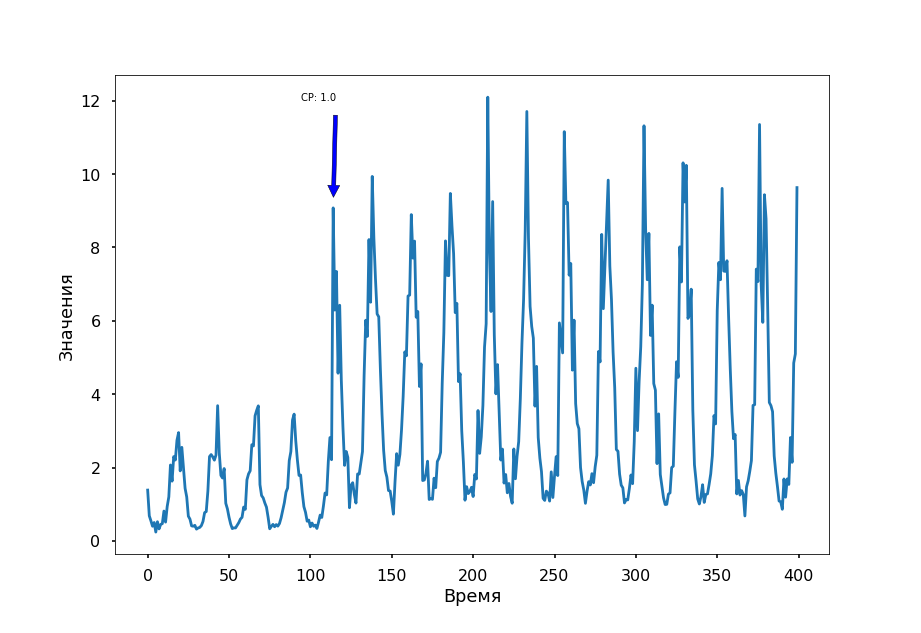
\includegraphics[width=12cm]{data_modeling_example_3}
%	\end{center}
%	\vspace{-5mm}\caption{Пример сгенерированного ряда с разладкой и мультипликативностью}
%	\label{fig:data_modeling_example_3}
%\end{figure}
%
%Как мы видим, за счет мультипликативности, в некоторых случаях ряд может слишком сильно изменяться --- вероятно нужно будет поменять некоторые параметры моделирования ряда, чтобы он стал больше похож на реальный ряд. Поэтому пока начнем с рядов без мультипликативности. В целом, результат похож на реальные ряды, поэтому пока будем двигаться дальше с такими параметрами моделирования.

%\todo[inline]{В качестве идеи на полях: можно ввести какую-то метрику схожести сгенерированных рядов и реальных.}


\section{Применение методов к моделированным данным и оценка качества этих методов}

\subsection{Сравнение методов с помощью ROC AUC}

Сгенерируем 50 рядов с локальной разладкой, 50 рядов с разладкой в среднем и 100 рядов без разладки. К каждому из этих рядов применим каждый из 7 методов (аппроксимация с моделями „среднее“, „косинус“, „4 косинуса“, „тренд“ и прогнозирование с моделями  „среднее“, „косинус“, „4 косинуса“) 15 раз (ко всем комбинациям из задержек $d = (4,24,48)$ и длин окон $l = (2,4,24,48,96)$. Результат будем оценивать по метрике ROC-AUC с 95\%-м доверительным интервалом. В таблице ~\ref{fig:results_pivot} изображены результаты ROC-AUC для всей решетки параметров и методов.

\begin{table}[!hhh]
	\caption{ROC AUC для разных методов}
	\begin{center}
		\vspace{-5mm}\includegraphics[width=18cm]{results_pivot}
	\end{center}
	\label{fig:results_pivot}
\end{table}

Как мы видим, метод аппроксимация с моделью „тренд“ сработал очень плохо для любых комбинаций параметров. Отсюда мы делаем первый вывод: если добавить в модель метода лишний, несвязанный с исходными данными компонент, то он испортит весь метод. Далее модель с трендом не будем рассматривать за ненадобностью.

Теперь сравним какой подход работает лучше: аппроксимация или прогнозирования. На рисунках ~\ref{fig:results_comparison_local}, ~\ref{fig:results_comparison_mean} изображены сравнительные графики ROC-AUC с 95\%-ми доверительными интервалами. Как мы видим, для любых комбинаций моделей и параметров доверительные интервалы аппроксимации и прогнозирования пересекаются. Это означает, что оба подхода работает примерно одинаково для условий нашей задачи. Поэтому далее будем рассматривать только один из этих подходов, например, аппроксимацию.

\begin{figure}[!hhh]
	\begin{center}
		\includegraphics[width=18cm]{results_comparison_local}
	\end{center}
	\vspace{-5mm}\caption{Сравнение ROC-AUC для локальной разладки}
	\label{fig:results_comparison_local}
\end{figure}

\begin{figure}[!hhh]
	\begin{center}
		\includegraphics[width=18cm]{results_comparison_mean}
	\end{center}
	\vspace{-5mm}\caption{Сравнение ROC-AUC для разладки в среднем}
	\label{fig:results_comparison_mean}
\end{figure}


Теперь сравним результаты друг с другом по сложности модели $f(x| \theta)$ в методе обнаружения разладки. Как мы видим из таблицы ~\ref{fig:results_pivot}, чем более точно модель описывает данные, тем лучше. При этом надо иметь в виду что лишние компоненты модели портят результат, поэтому следует усложнять модель только тогда, когда вы уверены что усложнение корректно.

Далее сравним результаты по длине окна $l$. Снова из таблицы ~\ref{fig:results_pivot} видно, что не кратные двум периодам окна работают хуже (потому что оценка происходит по неполной периодичности). При этом, очень маленькие окна работают достаточно хорошо, но только для локальной разладки.

С точки зрения задержки $d$, задержка для маленьких окон ухудшает качество метода при росте задержки. Но для больших окон эффект обратный --- наблюдается улучшение при росте задержки. 

Если сравнивать между собой качество на локальной разладке и на разладке в среднем, то видно следующее. Общая модель „среднее“ хорошо работает для обнаружения локальной разладки, но плохо работает для обнаружения разладки в среднем. При этом, более сложные модели хорошо работают для любого типа разладки. Следовательно, с разумно подобранной моделью можно обнаруживать оба типа разладки.

\subsection{Способ выбора порога $\gamma$}

Поскольку цель работы --- выработка рекомендаций по применению методов обнаружения разладок к реальным данным, то необходимо еще исследовать подходы к выбору разумного порога $\gamma$. Для этого выберем одну модель с одной конфигурацией параметров, которая показала хороший результат выше --- это будет аппроксимация с 4 косинусами, длиной окна $l=48$, задержкой $d=4$ и локальным видом разладки. Сгенерируем 1000 рядов без разладок и применим эту модель для расчета функции разладки. Далее, имея большой набор значений функции разладки мы можем взять некоторое значение из этого набора и принять его за порог $\gamma$. По сути этот набор значений является эмпирическим распределением функции разладки для ряда без разладки.  Вариантов здесь может быть несколько, попробуем протестировать следующие варианты:
\begin{itemize}
	\item 0.75 квантиль
	\item 0.95 квантиль
	\item Среднее + 2 стандартных отклонения
	\item Максимум
\end{itemize}



Результаты приведены в таблице ~\ref{fig:results_threshold_wo_cp}. Как видно, 0.75 квантиль позволяет найти практически все разладки, однако точность (в смысле ложно-положительных срабатываний) из-за этого сильно страдает. Если взять 2 стандартных отклонения или максимум, то точность будет очень высокая, однако количество обнаруженных разладок существенно упадёт. Поэтому в данном случае хорошим балансом между точностью и количеством обнаруженных разладок можно считать подход с 0.95 квантилью.

\begin{table}[!hhh]
	\caption{Качество метода, при разных подходах к заданию порога (ряды без разладок)}
	\begin{center}
		\vspace{-5mm}\includegraphics[width=7cm]{results_threshold_wo_cp}
	\end{center}
	
	\label{fig:results_threshold_wo_cp}
\end{table}


Однако в реальной жизни у нас не всегда есть длинный ряд, в котором мы уверены что не было разладок. Поэтому попробуем провести другой эксперимент: сгенерировать другие 500 рядов с разладкой и еще 500 рядов без разладки, посчитать функции разладок для каждого из этих рядов, получить эмпирическое распределения для значений функции разладки и далее применить те же подходы к выбору оптимального порога.

В результате получилось то, что изображено в таблице ~\ref{fig:results_threshold_cp}. Из выбранных нами подходов ни один не показал сбалансированного результата (все либо смещены в сторону точности, либо в сторону количества обнаруженных разладок). Поэтому попробуем посчитать качество при 0.80 квантиле. В таблице ~\ref{fig:results_threshold_cp_80} изображен результат --- получился хороший баланс между точностью и количеством обнаруженных разладок. Соответственно, практическая рекомендация будет следующая --- взять все имеющиеся исторические ряды (с разладкой и без), посчитать по ним функцию разладки и выбрать 0.80 квантиль от полученных значений как порог $\gamma$ для классификатора.

\begin{table}[!hhh]
	\caption{Качество метода, при разных подходах к заданию порога (ряды с разладкой)}
	\begin{center}
		\vspace{-5mm}\includegraphics[width=7cm]{results_threshold_cp}
	\end{center}
	
	\label{fig:results_threshold_cp}
\end{table}

\begin{table}[!hhh]
	\caption{Качество метода, при разных подходах к заданию порога (ряды с разладкой)}
	\begin{center}
		\vspace{-5mm}\includegraphics[width=7cm]{results_threshold_cp_80}
	\end{center}
	
	\label{fig:results_threshold_cp_80}
\end{table}

%Сгенерируем 100 рядов со случайной величиной разладки $\delta$ и случайным шумом $e$ и применим к каждому из этих рядов метод обнаружения разладки на основе аппроксимации. Функцию аппроксимации возьмем константную $\theta = (b)$, ширину окна $l = 48$, а порог $\gamma$ будем брать в диапазоне от $0$ до $1$ с шагом $0.01$. Пример функции разладки для данного метода с такими параметрами изображен на рисунке  ~\ref{fig:approximation_mean_1}. При этом, в качестве приемлемой задержке возьмем $u = 48$. Это означает, нотификация с запаздыванием в двое суток является для нас приемлемой, что, разумеется, не всегда верно в реальных задачах.
%
%\begin{figure}[!hhh]
%	\begin{center}
%		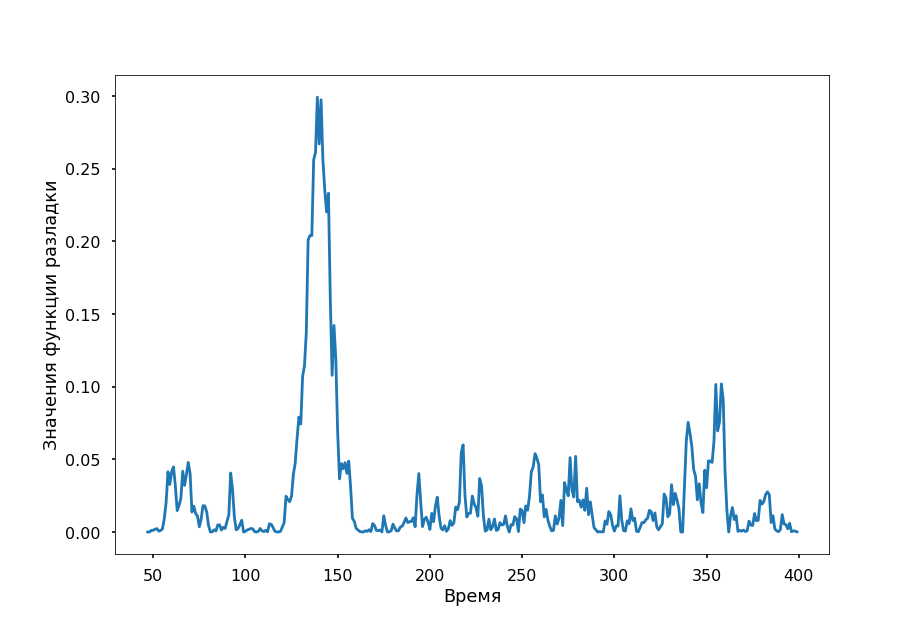
\includegraphics[width=12cm]{approximation_mean_1}
%	\end{center}
%	\vspace{-5mm}\caption{Пример функции разладки для сгенерированного ряда с разладкой и без мультипликативности}
%	\label{fig:approximation_mean_1}
%\end{figure}
%
%Для тысячи рядов с заданными параметрами метода обнаружения разладки и заданным диапазоном порога ROC-кривая получилась следующая (рисунок ~\ref{fig:approximation_mean_2_roc}). ROC-кривая проходит довольно далеко от базовой линии, что говорит о том, что в целом метод с такими параметрами работает уже достаточно хорошо (разумеется, надо понимать, что пока что мы взяли приемлемую задержку равную 48 часам, что является очень мягкими условиями эксперимента, в сравнении с реальной жизнью). 

% Во-вторых, мы видим нетипичное для ROC-кривой поведение в верхнем правом углу: кривая уходит под базовую линию. Дело всё в том, что это происходит только в случае очень низких порогов и связано с моментом обнаружения разладки. Каждый раз после обнаружения разладки в ряде, метод начинает искать следующую разладку начиная с точки последней разладки (как бы отрезая и не учитывая данные, которые были до последней разладки). Это приводит к тому, что если разладка случайно обнаружилась (а при низком пороге это типичная ситуация) незадолго до фактической разладки, то скорее всего сама разладка не будет обнаружена. Этим объясняется почему, при очень низком пороге может быть True positive rate существенно ниже 1.


%\begin{figure}[!hhh]
%	\begin{center}
%		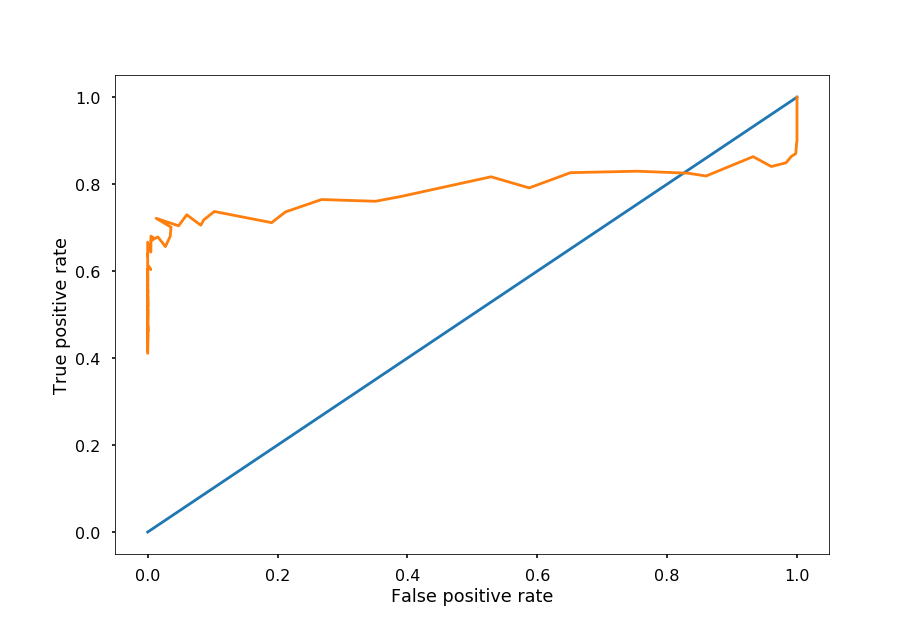
\includegraphics[width=12cm]{approximation_mean_2_roc}
%	\end{center}
%	\vspace{-5mm}\caption{ROC-кривая для 1000 смоделированных рядов и метода на основе аппроксимации}
%	\label{fig:approximation_mean_2_roc}
%\end{figure}
%
%Попробуем применить метод обнаружения разладки на основе прогнозирования к такой же тысяче рядов. Параметры метода будем брать аналогичными параметрам аппроксимации (кроме порога). 
%Функция прогнозирования константная $\theta = (b)$, ширина окна $l = 48$, индекс разделения окна $g = 24$, порог $\gamma$ будем брать в диапазоне от $0$ до $5$ с шагом $0.05$.
%
%Получившийся результат представлен на рисунке ~\ref{fig:roc_pred_approx}. Как видно из ROC-кривых с данными параметрами метод на основе аппроксимации сработал лучше, нежели метод на основе прогнозирования. Безусловно, требуется настройка параметров, как для моделирования данных, так и для самих методов, но цель работы --- создать стенд для проверки идей и гипотез по обнаружению разладок --- достигнута, поскольку нам удалось сравнить качество двух разных методов в контролируемом эксперименте.

%\begin{figure}[!hhh]
%	\begin{center}
%		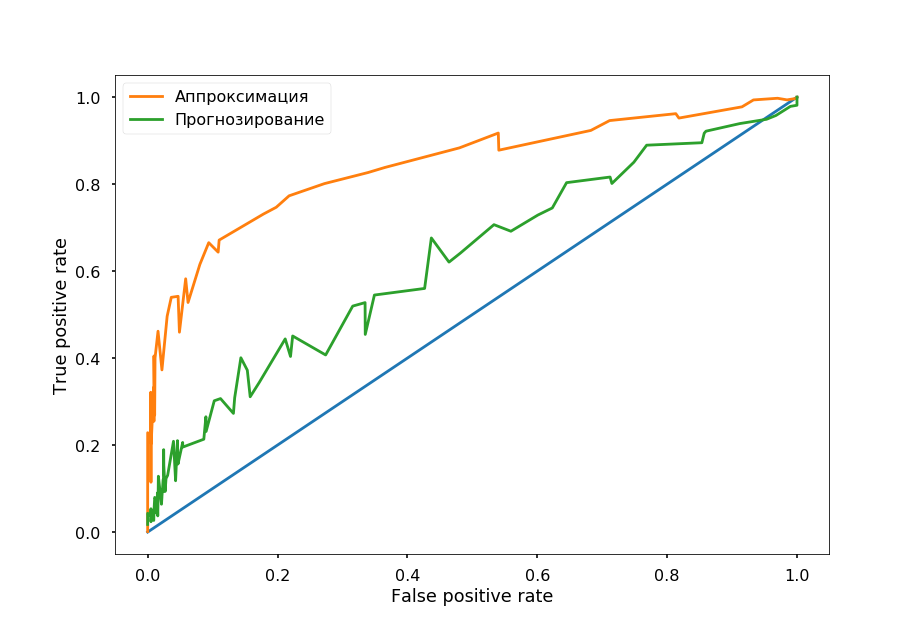
\includegraphics[width=12cm]{roc_pred_approx}
%	\end{center}
%	\vspace{-5mm}\caption{ROC-кривые для 1000 смоделированных рядов}
%	\label{fig:roc_pred_approx}
%\end{figure}


\conclusion
В данной работе мы установили подход к моделированию временных рядов показов мобильной рекламы, формально описали некоторые методы обнаружения разладки и описали способ оценки качества методов обнаружения разладки во временных рядах. Во второй части работы, мы применили описанные методы к сгенерированным данным и сравнили качество методов. Помимо этого, мы выработали подход к определению оптимального порога и протестировали качество такого подхода в эксперименте. В результате были получены рекомендации по использованию методов обнаружения разладки и выборе параметров этих методов.

%$$ P \cos(\frac{2\pi}{p}x + \phi) = \sum_{j=1}^r c_j \mu_j^n $$

%\bibliography{bibliography}
\bibliography{reference}
%\bibliography{otchet}


% Не добавлять длинное тире в качестве разделителя
%\newcommand\BibDash{}
% Выделять курсивом
%\let\BibEmph=\emph
%\bibliographystyle{gost2008}

% Список литературы
% \bibliography{thesis}


%\begin{thebibliography}{9}
%	\bibitem{ssa_forecast} Голяндина Н.Э. Метод „Гусеница“-SSA: прогноз временных рядов. Учебное пособие. СПб., 2003.
%	\bibitem{armstrong} Armstrong. Principles of Forecasting: A Handbook for Researchers and Practitioners. Kluwer Academic Publishers, 2001.
%	\bibitem{dagum} Dagum, Estela, Bianconcini. Seasonal Adjustment Methods and Real Time Trend-Cycle Estimation, 2016.
%	\bibitem{ssa_book} N. Golyandina, V. Nekrutkin, A. Zhigljavsky. Analysis of Time Series Structure - SSA and Related Techniques, 2001.
%	\bibitem{hyndman} R. Hyndman, G. Athanasopoulos. Forecasting: Principles and Practice. 2013.
%	\bibitem{moving_average} R. Hyndman. Moving averages. 2009.
%	
%\end{thebibliography}

% Приложения
\appendix



\end{document}
